\documentclass[journal]{IEEEtran}
\usepackage[a5paper, margin=10mm, onecolumn]{geometry}
\usepackage{amsmath,amssymb,amsfonts,amsthm}
\usepackage{mathtools}
\usepackage{gvv-book}
\usepackage{gvv}
\usepackage{hyperref}

\begin{document}

\title{4.13.50}
\author{Puni Aditya - EE25BTECH11046}
\maketitle

\textbf{Question:}

Two equal sides of an isosceles triangle are given by the equations $7x - y + 3 = 0$ and $x + y - 3 = 0$ and its third side passes through the point $(1, -10)$. Determine the equation of the third side.

\textbf{Solution:}
Let the two equal sides of the isosceles triangle be represented by
\begin{align*}
    \vec{n_1}^\top\vec{x} &= c_1 \\
    \vec{n_2}^\top\vec{x} &= c_2
\end{align*}
and the third side by the line
\begin{align*}
    \vec{n}^\top\vec{x} &= c
\end{align*}
For a line passing through a given point $\vec{p}$,
\begin{align}
	\vec{n}^\top\vec{x} &= \vec{n}^\top\vec{p} \\
    \text{Here, }\vec{p} &= \myvec{1 \\ -10}
\end{align}
The third side of the isosceles, the base, is perpendicular to one of the angle bisector of the two equal sides and parallel to the other.
\begin{align}
    \vec{m_1} &= \frac{\vec{n_1}}{\norm{\vec{n_1}}} + \frac{\vec{n_2}}{\norm{\vec{n_2}}} \label{eq:31} \\
    \vec{m_2} &= \frac{\vec{n_1}}{\norm{\vec{n_1}}} - \frac{\vec{n_2}}{\norm{\vec{n_2}}} \label{eq:32}
\end{align}
Hence,
\begin{align}
	\vec{n} = \vec{m_2}\text{ or }\vec{n} = \vec{m_1}
\end{align}
For the given question,
\begin{align}
    \vec{n_1} &= \myvec{7 \\ -1}\text{ and }\vec{n_2} = \myvec{1 \\ 1} \\
    \norm{\vec{n_1}} &= \sqrt{50} = 5\sqrt{2} \\
    \norm{\vec{n_2}} &= \sqrt{2}
\end{align}
For the side parallel to $\vec{m_2}$, using \eqref{eq:31},
\begin{align}
    \vec{n} &= \frac{1}{5\sqrt{2}}\brak{\myvec{7 \\ -1} + \myvec{5 \\ 5}} = \frac{1}{5\sqrt{2}}\myvec{12 \\ 4} \\
    \vec{n} &= \myvec{3 \\ 1} \\
    \myvec{3 & 1}\vec{x} &= \myvec{3 & 1}\myvec{1 \\ -10} \\
	\myvec{3 & 1}\vec{x} &= -7
\end{align}
For the side parallel to $\vec{m_1}$, using \eqref{eq:32},
\begin{align}    
    \vec{n} &= \frac{1}{5\sqrt{2}}\brak{\myvec{7 \\ -1} - \myvec{5 \\ 5}} = \frac{1}{5\sqrt{2}}\myvec{2 \\ -6} \\
    \vec{n} &= \myvec{1 \\ -3} \\
	\myvec{1 & -3}\vec{x} &= \myvec{1 & -3}\myvec{1 \\ -10} \\
    \myvec{1 & -3}\vec{x} &= 31
\end{align}

\begin{figure}[h!]
	\centering
	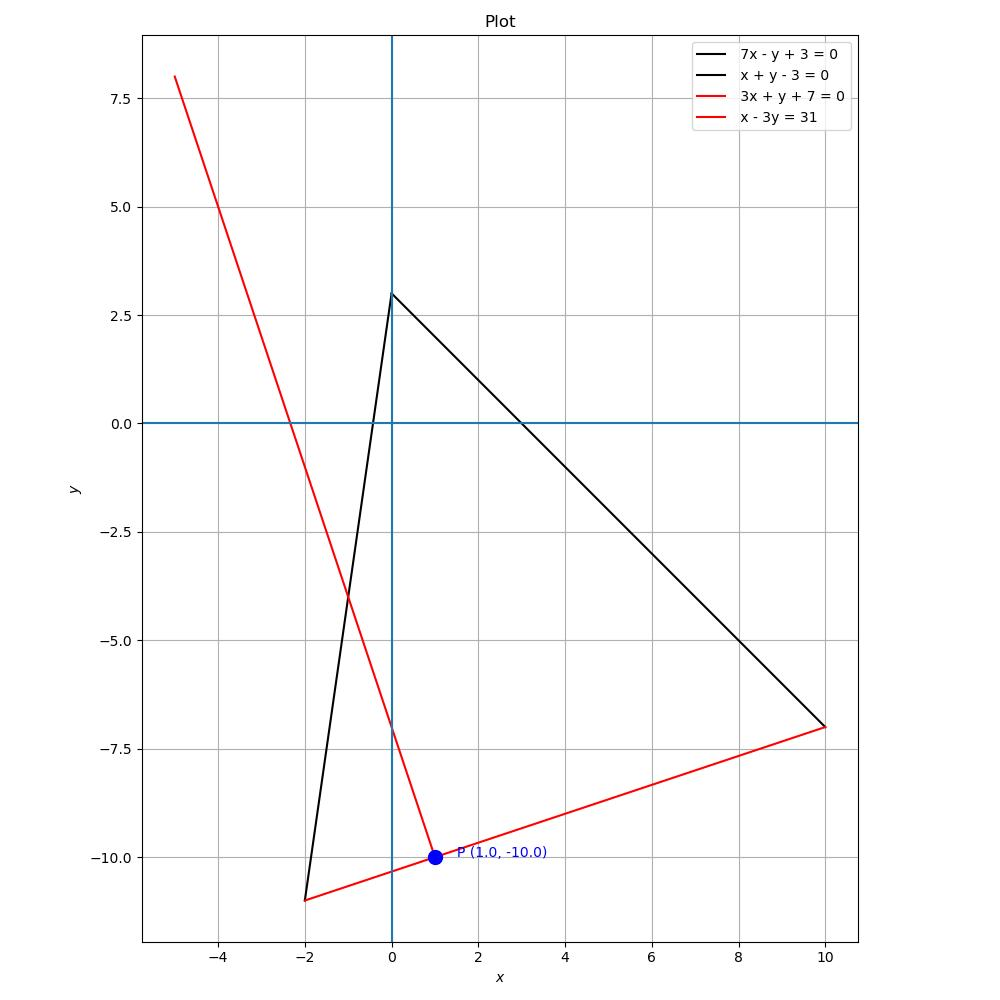
\includegraphics[width=0.6\columnwidth]{figs/plot_c.jpg}
	\caption*{Isosceles Triangle}
	\label{fig:fig}
\end{figure}

\end{document}
